\documentclass[12pt]{article}
\usepackage{fullpage,graphicx,psfrag,amsmath,amsfonts,verbatim}
\usepackage[small,bf]{caption}

\input defs.tex

\bibliographystyle{alpha}

\title{
CS 230 Project Proposal: Developing a hybrid filter for bandlimited signals using neural networks
\newline 
\newline
Project Category: Supervised Learning, modelling, signal processing
}
\author{Jonathan Tuck}

\begin{document}
\maketitle

\newpage
\tableofcontents
\newpage

\section{Introduction}
In the field of signal processing, filtering is among the most ubiquitous of topics.
Typically, when one wants to filter a signal, one must know what type of filtering should be done
(\ie, low-pass filtering, high-pass filtering, \etc,) which also implicitly
requires the prior knowledge of the bandwidth of the signal. Unfortunately, unknown
signals' bandwidths are typically only found by computing their Fourier transform and observing
a steep dropoff in magnitude for a given frequency. Currently, the method of computing a Fourier transform
for a discrete signal can be computed in $O(n \log n)$ time \cite{B:78,O:17}.

The goal of this project is to use a neural network to create a multi-purpose filter for use in
signal processing topics. This neural network should be able to determine the bandwidth of any signal
that is input, without having to compute the Fourier transform.

\section{Background}
The context and background for this project is abundant, as signal processing has enjoyed a vast treatment
in the past century. The Fourier series for a signal \cite{B:78,O:17} is
\BEQ
f(t) = \sum_{n=-\infty}^{\infty} c_n e^{2 \pi i n t / T}.
\EEQ
Here, we refer to $T$ as the \textit{period} of the signal, $c_n$ as the $n$-th 
\textit{Fourier coefficient}, and $e^{2 \pi i n t / T}$ as the $n$-th \textit{harmonic}.
In addition, if the coefficients 
$\{c_n\}_{n=-\infty}^{\infty} = 0$ for some $|n| > B/2,$ then we say that the signal is 
\textit{bandlimited} with \textit{bandwidth} $B.$

Figure \ref{f-example_bandlimited} below illustrates a simple example of a signal bandlimited to 2200 Hz,
and its Fourier transform $F(s).$

\begin{figure}[ht]
\begin{center}
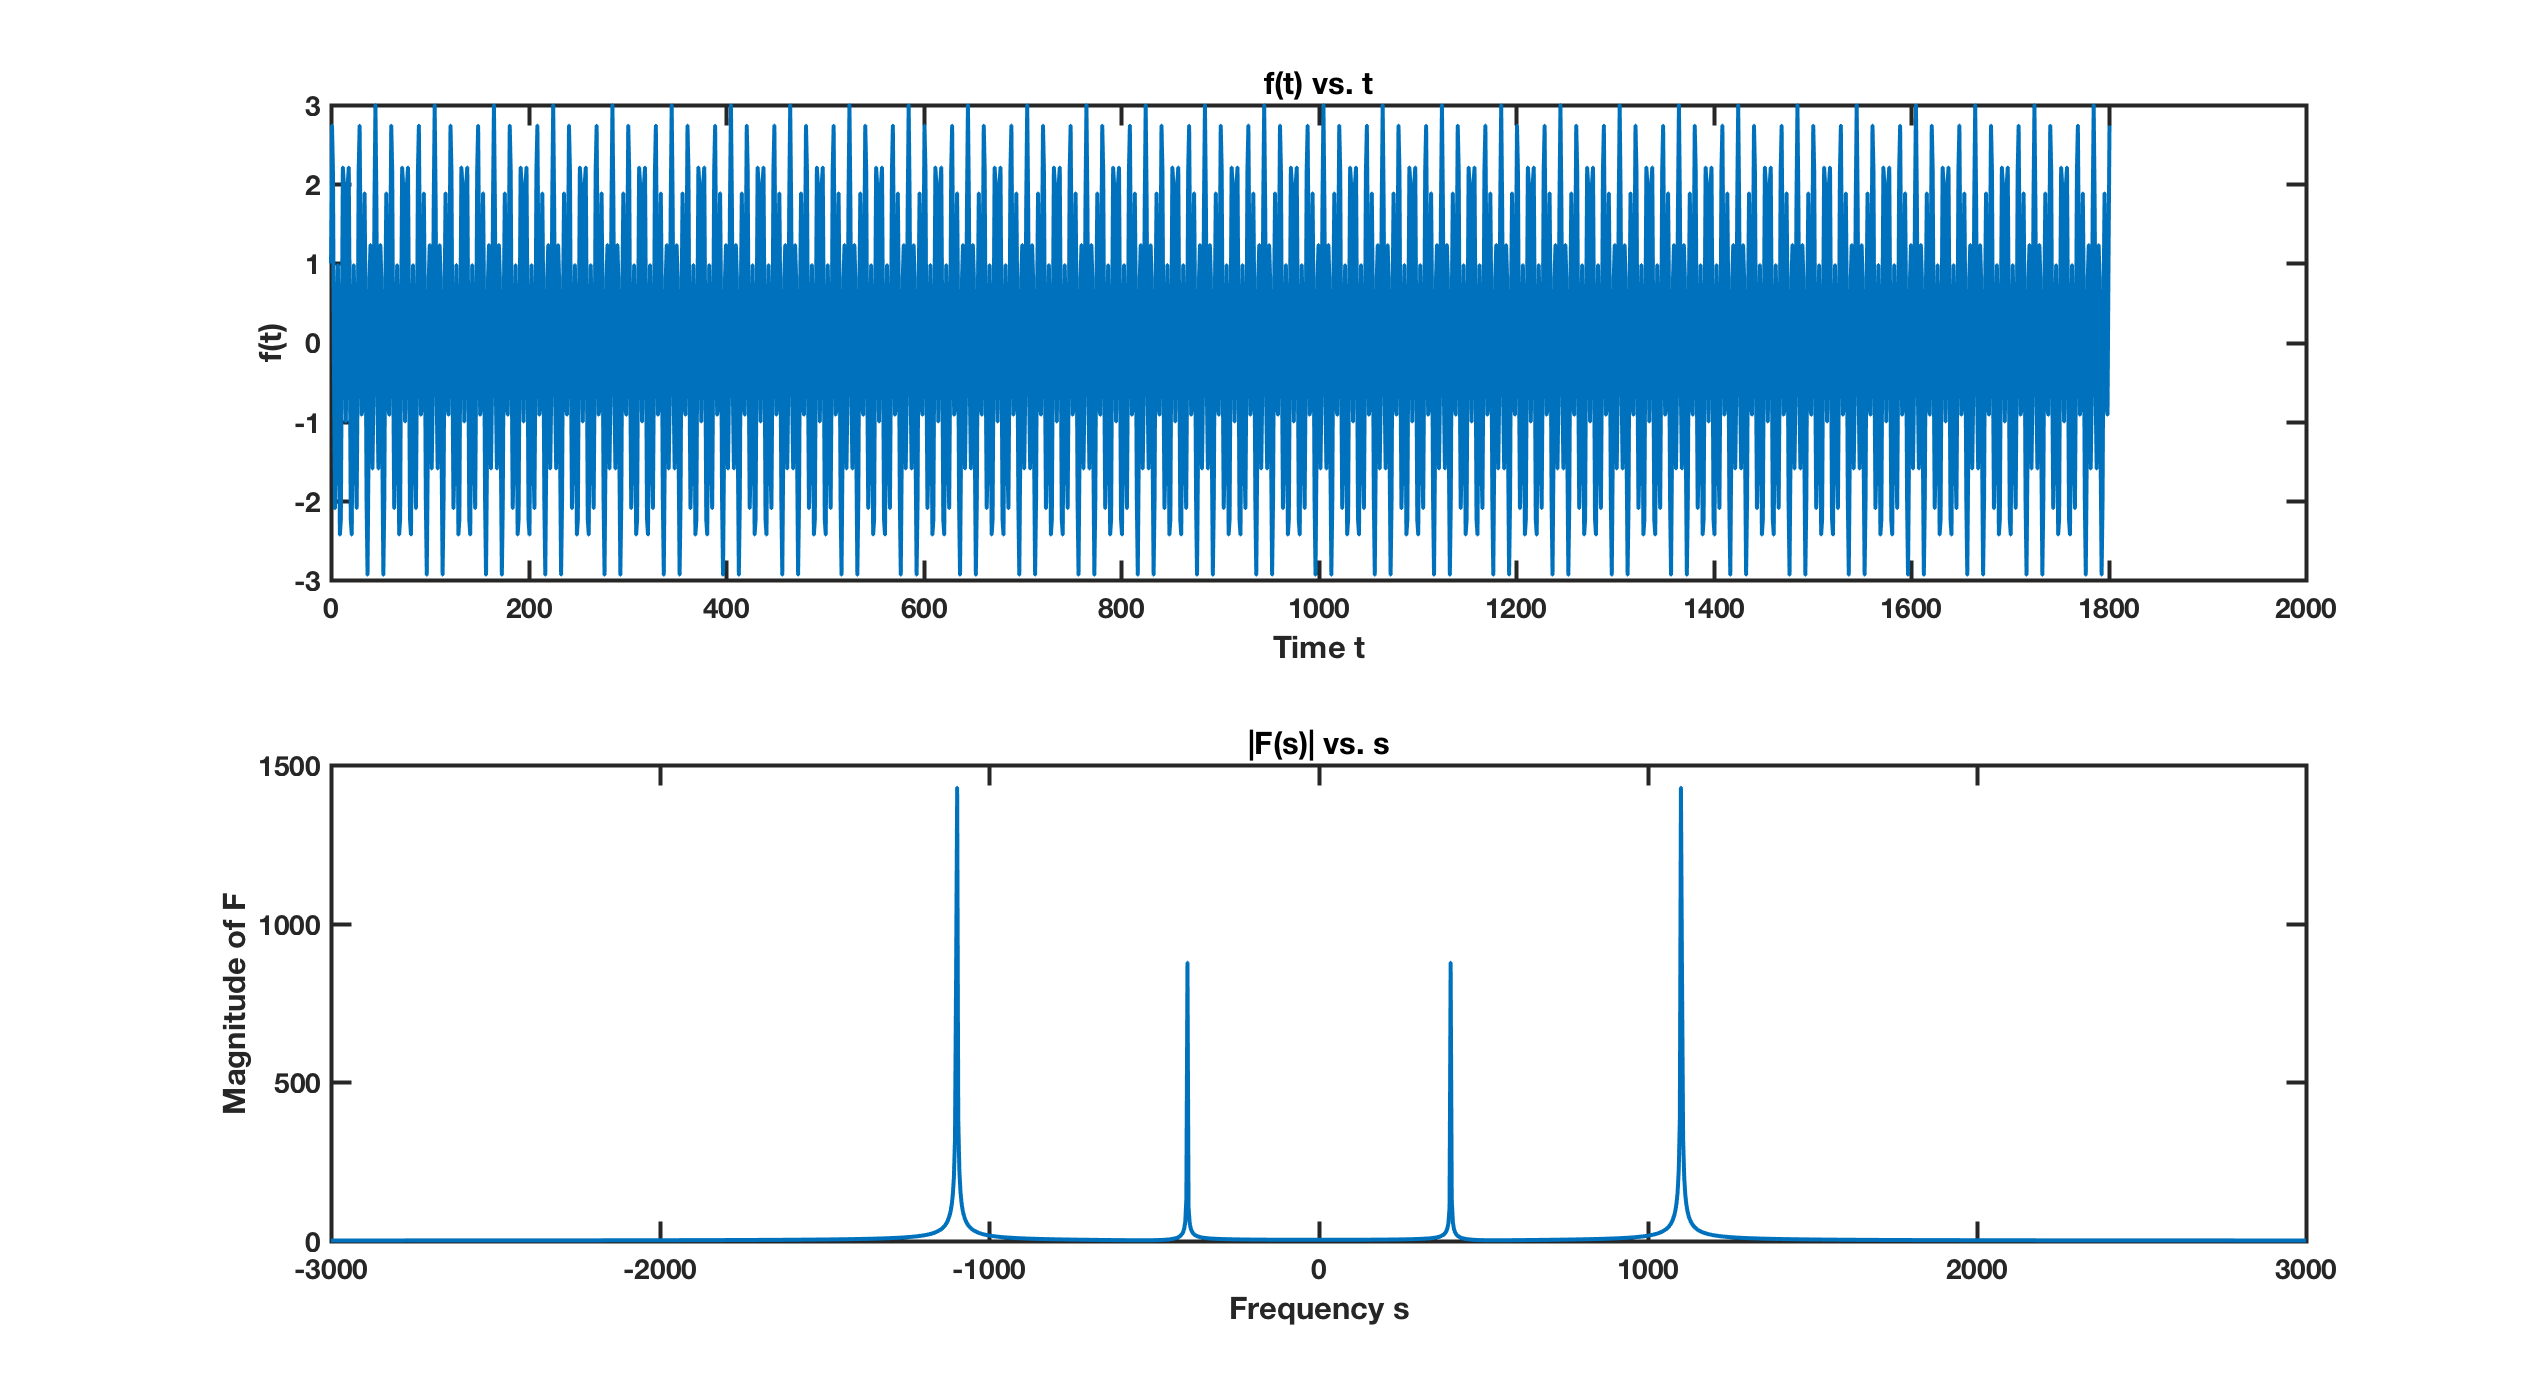
\includegraphics[width=.9\textwidth]{figures/example_bandlimited.png}
\end{center}
\caption{Bandlimited signal $f(t) = \cos(800 \pi t) + 2\sin(2200 \pi t)$ and the magnitude of its Fourier transform.}
\label{f-example_bandlimited}
\end{figure}

In the past, the typical method for determining the bandwidth of a signal has been by inspection of that
signal's Fourier transform. The Fourier transform $F: \reals \rightarrow \reals$ of a signal $f(t)$ is 
defined as
\BEQ
F(s) = \int_{-\infty}^{\infty} e^{-2 \pi i s t} f(t) dt.
\EEQ

\section{Challenges}
In an ideal world, bandlimited signals would be clean; there would be no signal past 
a particular bandwidth. Unfortunately, we might sometimes encounter noise of various forms 
in our signal. One of the larger challenges in this project is to build the neural network 
to recognize when a small magnitude is either noise or a portion of the whole signal.

\section{Data}
An advantage of this project is that the data is readily abundant and training data can be
synthetically generated efficiently. Since all signals are simply sums of sinusoids at different
frequencies and amplitudes, we will generate our data by adding randomly generated sinusoids together, 
some with various types of noise. For each example, we shall randomly choose the number of sinusoids 
to be added, their frequencies, and their amplitudes.

\section{Method and implementation}
The problem of determining the bandwidth of a signal is a supervised learning problem, and so
neural networks for supervised learning problems will be used. We do not yet know the appropriate
deep learning architecture for this project, but as the act of convolution is deeply related to Fourier 
transforms \cite{B:78,O:17}, we shall attempt to use architectures such as convolutional neural networks 
\cite{LBBH:98,RSA:15}.

\section{Evaluation metrics}
The evaluation of this project shall be based on how close the neural network estimates for 
a signal's bandwidth are to the actual signal's bandwidth. The metric to be evaluated is
\[
E_1 = (1/m) \sum_{i=1}^{m} \ones\{|B^{(i)} - \hat B^{(i)}| > \epsilon\},
\]
where $m$ is the number of samples in the set, 
$\ones : \reals \times \reals \times \reals \rightarrow \reals$ is the 0-1 indicator function, 
$B$ is the actual signal bandwidth, $\hat B$ is the signal bandwidth estimate,
and $\epsilon > 0$ is some small tolerance to be chosen.

\newpage
\bibliography{template}

\end{document}
